\documentclass{article}
\usepackage[utf8]{inputenc}

\usepackage{graphicx}
\usepackage{float}
\usepackage{enumerate}
\usepackage{hyperref}
\hypersetup{
colorlinks=true,
linkcolor=blue,
filecolor=magenta, 
urlcolor=blue,
}

\urlstyle{same}

\title{Project Imacs: Development Process Document}
\author{Group 16:\\ Kelvin Lin\\ Jiahong Dong\\ Liam Casola\\ Varun Hooda\\ Mikolaj Hrycko\\ Danish Khan\\ Prince Sandu\\ Baltej Toor}
\date{November 30\textsuperscript{th} 2018}

\begin{document}

\maketitle
\newpage
\tableofcontents
\newpage

\section{Process Workflow}
\label{sec:process-workflow}
The following documents Team 16's workflow processes. Since Project Imacs is a fully software-based project, all of the subsystems will be designed, implemented, and tested in a similar fashion outlined in this section. Project Imacs is split into 4 core features: the file management system, handwriting recognition and general inputs, data visualization, and user experience. Team members are split such that each pair of student "owns" one of the 4 core features, or a key aspect of overall software architecture design. Ownership is defined as the responsibility for ensuring that an appropriate amount of work is put into completing the feature by the overall team. All team members are expected to contribute to all 4 features, as expalined in \hyperref[sec:roles-responsibilities]{Roles and Responsibilities}.

\subsection{Overview}
\label{sec:process-overview}
All progress made in Team 16 begins with communication between team members through a weekly meeting or through the online messaging platform Gitter. Once issues or opportunities have been identified, a issue ticket is created on Github's issue tracking software, and it is assigned to a team member based on pre-assigned responsibilities to oversee its completion. The assigned team member will be responsible for completing the assigned task, or decomposing it into smaller tasks and assigning it to other members. In completing the issue, the team member may use a variety of tools including, but not limited to, textbooks references for designing the software, a programming language (e.g. HTML, CSS, JavaScript, TypeScript) and an Integrated Development Environment for software development, and a web browser as well as automated testing tools for software testing. Once the assigned task is completed, it is reviewed by 2 members of the team, randomly selected, who did not participate in resolving the issue ticket. The team member assigned to the issue ticket is responsible for making any suggested changes by the 2 reviewers. Once the reviewers are satisified with the changes, then the work is merged into the master branch where all of the final source code and documentation is stored.

\subsection{Tools Used}
The tools that Team 16 expects to use are listed below. As the project evolves, additional tools may be introduced. All tools used shall be the latest publicly available stable version, unless otherwise noted.

\subsubsection{Communication and File Sharing}
Communication and file sharing tools are used to facilitate asynchronous communication among team members, and to allow for the remote transfer of files. The following tools will be used:

\begin{itemize}
\item Gitter: Used for team-wide communication between team members.
\item Email: Used for formal communication between Team 16, the professor, and the TAs.
\item Google Drive: Used for sharing drafts of documentation before they are formalized. Google Drive also allows for collaborative real-time work.
\item Google Hangouts: Used for video conferencing in the event of bad weather or if an emergency meeting is needed.
\end{itemize}

\subsubsection{Text Editors}
Text editors are used to develop documentation for Project Imacs. The following text editors will be used:

\begin{itemize}
\item LaTeX: Used for writing formal documentation, as defined in \hyperref[sec:formal-documentation]{Writing Formal Documentation}.
\item Google Docs: Used for writing informal documentation, as defined in \hyperref[sec:informal-documentation]{Writing Informal Documentation}.
\item Microsoft Word: Used for writing informal documentation.
\item Markdown: Used for writing informal documentation.
\end{itemize}

\subsubsection{Integrated Development Environments}
Integrated Development Environments (IDEs) facilitate the development of software. The following IDEs will be used:

\begin{itemize}
\item Visual Studio Code: Used for intensive coding tasks as it contains advanced features to assist with software development.
\item Vim: Used for coding when the changes are minor or if the task needs to be completed quickly on a resource limited machine.
\end{itemize}

\subsubsection{Issue Tracking}
Issue tracking software is used to track tasks that need to be completed, issues identified, or changes that need to be made. The following software will be used for issue tracking:

\begin{itemize}
\item Github Issue Tracking: Used to keep track of tasks that need to be completed, and for assigning team members to be responsible for certain tasks.
\end{itemize}

\subsubsection{Programming, Markup, and Scripting Languages}
Programming, markup, and scripting languages are used to develop software for Project Imacs. The following languages will be used:

\begin{itemize}
\item HTML: Used for creating webpages and user interfaces.
\item CSS: Used to style user interfaces.
\item JavaScript: Used for programming features for Project Imacs.
\item TypeScript: Used for programming features for Project Imacs.
\end{itemize}

\subsubsection{Package Managers}
Package managers allow external software packages and libraries to be integrated into the software without having to manually install each package. Package managers can also ensure that each team member will download the appropriately versioned required packages for the project. The following package manager will be used:

\begin{itemize}
\item Node Package Manager: Used to automatically organize and install the appropriate JavaScript/NodeJS libraries for each team member.
\end{itemize}

\subsubsection{Version Control}
Version control will be used to organize team workflow and track all changes made to Project Imacs. The following version control software will be used:

\begin{itemize}
\item Git: Used for tracking all updates and changes made to Project Imacs. More information is available in the \hyperref[sec:version-control]{Version Control} section.
\end{itemize}

\subsection{Identifying an Issue, Change, or Opportunity}
\label{sec:issues-opportunity}
As the project progresses, issues and opportunities will become apparent and team members will be expected to address them. To keep track of all issues and opportunities, Github's issue tracking software will be used. Github's issue tracking software allows for issue tickets ("issues") to be created and assigned to team members who will be responsible for overseeing its completion. The steps to identifying an issue or opportunity is as follows:

\begin{enumerate}
\item Discuss the potential issue or opportunity with the team either during the weekly meeting described in \hyperref[sec:hold-meeting]{Holding a Meeting}, or through freeform communication through the team's online messaging platform, Gitter.
\item Create an issue on Github's issue tracking software with complete details describing the issue or opportunity, and the deliverables required to mark the issue as complete.
\item Assign the appropriate team member(s) to oversee the completion of the task, according to the \hyperref[sec:roles-responsibilities]{Roles and Responsibilities} section.
\end{enumerate}

By the end of these steps, a meaningful issue should be created on Github's issue tracking software, and the appropriate team members should be aware of the issue.

\subsection{Holding a Meeting}
\label{sec:hold-meeting}
Meetings are to be held during the first SFWRENG 4G06 time slot without a scheduled meeting with the professor or the TAs. Meetings will be held in an ITB capstone workroom, and the BSB lecture room will be used if there is no space available in ITB. All members are expected to be present, prepared, and to meaningfully contribute during the meetings. The meetings will be held according to the following steps:

\begin{enumerate}
\item Everyone sits in a circle facing towards the center such that everyone can see and hear each other.
\item Kelvin will update everyone of the upcoming deliverables required for the course, and team members will be assigned tasks to complete the required deliverable.
\item Varun will update everyone of the technical tasks related to the implementation of Project Imacs, and team members will be assigned tasks to help further its development.
\item Going around the circle, each team member will talk about what they worked on, what they need help with, and what they will do the following week. If a team member encounters difficulties that can be resolved by another team member, then the issue will be jointly assigned to the two team members.
\item All team members will be asked if they would like to add anything or ask any questions before the meeting ends.
\item The meeting is adjourned.  
\end{enumerate}

At the end of every meeting, all team members are expected to know what the required deliverables are for that week, and what tasks they are expected to complete.

\subsection{Writing Formal Documentation}
\label{sec:formal-documentation}
Documentation will need to be written to facilitate communciation, complete course deliverables, and enable knowledge transfer within the team. Formal documentation is defined as any document that satisfies one or more of the following conditions: consistent formatting is important for continuity with a previous document, there is a high likelihood that the document will need to be compatible with a future document, the document was previously an informal document that became formal later on, the document is a course deliverable and it is longer than 1 page, or the document is a course deliverable worth more than 1\% of the final grade. This definition implies that a previously informal document may become formal later on, and when it becomes formal, it must be properly converted.

The following steps outline the procedure for writing formal documentation:

\begin{enumerate}
\item Ensure a full understanding of the task-at-hand before starting. Ask any questions needed to better understand what is required.
\item Create a document on Google Drive and create an outline for the deliverable.
\item Fill in the outline.
\item Send a message on Gitter and ask other team members to contribute by adding additional content and editing existing content.
\item Pull from the \texttt{docs} Git repository.
\item Create a folder for the new document following the \hyperref[sec:git-conventions]{Git Standards and Conventions}.
\item Create a new LaTeX file in the folder.
\item Properly convert the Google Drive document into LaTeX, ensuring that the formatting is appropriate for the document, and is reasonably consistent with any previous documents.
\item Push the change into the Git repository.
\item Send a message on Gitter and ask other team members to contribute by adding additional content and editing existing content.
\end{enumerate}

\subsection{Writing Informal Documentation}
\label{sec:informal-documentation}
Informal documentation is defined as any document that is not formal. Informal documentation will primarily be used for internal purposes, and will have little impact, if any, on the course grading. While the quality of the content should be on par with the quality of a formal document, the difference between a formal document and an informal document is that an informal document does not need to have consistent styling with other documents, so that the informal document can be produced in a faster manner.

The following steps outline the procedure for writing informal documentation:

\begin{enumerate}
\item Ensure a full understanding of the task-at-hand before starting. Ask any questions needed to better understand what is required.
\item Open a text editor (e.g. Google Docs, Microsoft Word, Markdown).
\item Write meaningful content into the text file.
\item Upload it to Google Drive.
\item Send a message on Gitter and ask other team members to contribute by adding additional content and editing existing content.
\end{enumerate}

Additionally, if the informal document is a course deliverable that is 1 page or shorter, and it is worth less than 1\% of the final course grade, then the following steps need to be taken:

\begin{enumerate}
\item Ensure that a reasonably sized serif font is used in the document.
\item Pull from the \texttt{docs} Git repository.
\item Create a folder for the new document following the \hyperref[sec:git-conventions]{Git Standards and Conventions}.
\item Put the document into the folder.
\item Push the new file into the Git repository.
\end{enumerate}

\subsection{Completing a Github Issue}
\label{sec:github-issue}
When an issue is assigned to a team member, the team member is responsible for overseeing its development, or for further decomposing the task into smaller tasks for other members. In the case of the latter, the assigned team member should reference \hyperref[sec:issues-opportunity]{Identifying an Issue or Opportunity}. In the case of the former, the following steps should be taken:

\begin{enumerate}
\item Ensure a full understanding of the task-at-hand before starting. Ask any questions needed to better understand what is required.
\item Create a design for the software to be developed, and show the design to the owner of the subsystem.
\item Pull the latest changes from the appropriate Git repository.
\item Create a branch off the master branch, and name it according to the \hyperref[sec:git-conventions]{Git Standards and Conventions}.
\item Update the "README" with a meaningful description of the task undertaken and steps needed to run or test the software.
\item Develop the software using an integrated development environment, and the most recent version of the API and programming languages. Adhere to the \hyperref[sec:code-standards]{Coding Standards and Conventions} outlined below.
\item Commit to the local branch whenever a milestone is reached.
\item Once the code is complete, tests should be run to ensure the code reasonably exhibits desired behaviour.
\item Create a pull request for the code to merge it into the master branch, and have it reviewed as per \hyperref[sec:reviewing-code]{Reviewing Code}.
\item Implement any suggestions by the reviewers.
\item Complete the merge into the master branch, and notify others through a message on Gitter.
\item Mark the Github issue as resolved.
\end{enumerate}

At the end of these steps, the Github issue task should be implemented into the offical Project Imac source code, and the Github issue should be marked as resolved.

\subsection{Reviewing Code}
\label{sec:reviewing-code}
When a coding task is complete as per \hyperref[sec:github-issue]{Completing a Github Issue}, it should be reviewed by 2 different members of the team who did not participate in resolving the issue. These two team members are randomly selected. The selected reviewers will take the following steps:

\begin{enumerate}
\item Ensure a full understanding of the assigned task. Ask any questions needed to understand the scope of the issue.
\item Pull the latest changes from the appropriate Git repository.
\item Test the code to ensure it runs and reasonably behaves as expected.
\item Review the code line by line to look for logical inconsistencies.
\item Review the code line by line to look for inconsistent styling.
\item Provide feedback to the team member assigned to task.
\item Iterate with the team member assigned to the task until the code is satisfactory and the changes have been merged into the master branch.
\end{enumerate}

By the end of these steps, the code should be reasonably consistent with the style guide, and it should reasonably behave as expected.

\section{Version Control}
\label{sec:version-control}
Project Imacs will use Git, hosted on Github, for version control. A Github organization will be created to host all of Project Imac's repositories.There will be two repositories within the project: one for storing Project Imac's source code, while another to host documentation. Team members are expected to concurrently work on their tasks by using separate branches, and then merging their changes back to the master brach by creating a pull request. Pull requests are to be reviewed by at least 2 members before they are merged into the master branch. These 2 members must be different than the team member who wrote the code. Furthermore, Github's Issue Tracking feature will be used to keep track of tasks, enhancements, and bugs for the projects. The issues created in the issue tracking software will be assigned to individual team members who will be responsible for overseeing the completion of the task.

\subsection{Repository Descriptions}
This section will provide a description of the repositories used in Project Imacs.

\subsubsection{Docs}
The \texttt{docs} repository is for documents and any research that is done. All notes from research should be uploaded as plain text files in the appropriate \texttt{research/} top-level directory. This file should ideally be a Markdown file (\texttt{research-foo.md}). Any demonstrations of an algorithm or API should also be located in the \texttt{research/} top-level directory.

\subsubsection{Dev}
The \texttt{dev} repository contains the source code for Project Imacs. The code in this repository should adhere to the following \hyperref[sec:git-conventions]{Git conventions}.

\section{Standards and Conventions}
\subsection{Git Standards and Conventions}
\label{sec:git-conventions}
\subsubsection{Creating and Managing Branches}
\begin{itemize}
\item Branches are to use the following naming convention: \texttt{feature/\{Name of the feature implemented\}}, \texttt{fix/\{Name of the fix implemented\}}, or \texttt{misc/\{Name of the task implemented\}}.
\item Branch names should follow the kebab-case naming convention.
\item The master branch is protected, and a pull request must be created in order to merge code into the master branch.
\end{itemize}

\subsubsection{Committing Code}
\begin{itemize}
\item Do not commit code into another team member's branch without first consulting that team member.
\item Always branch from the most recent version of another branch.
\item Commit messages should not be more than 50 characters.
\item Commit messages should follow the \href{https://commit.style}{commit.style} style guide.
\item A commit body is encouraged but optional. Either paragraphs or bullet points in the commit body are acceptable.
\item Use \texttt{git add -p; git commit -vv} when committing code to carefully review the items to be commited and to provide a good commit message.
\item Compiler generated code should not be committed, and their extensions should be included in the Gitignore file. Each team member is expected to generate files from the source on their own machines.
\item Do not commit any sensitive information (e.g. student ID numbers) or API keys to any Git repository.
\item Do not commit any breaking changes to Git.
\end{itemize}

Examples of acceptable and unacceptable commit messages are shown below:

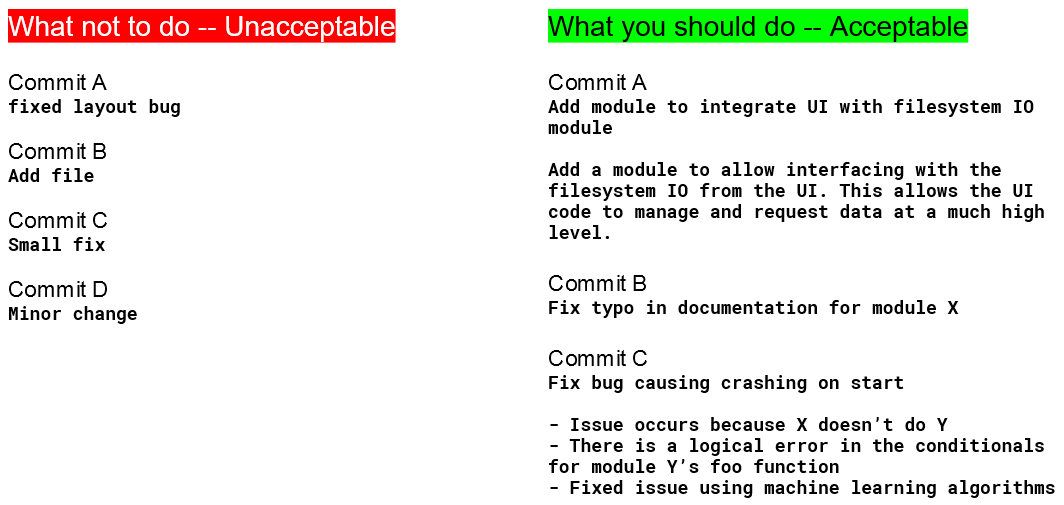
\includegraphics{git-example.png}

\subsection{Coding Standards and Conventions}
\label{sec:code-standards}
\begin{itemize}
\item 2 space indents should be used for web-development languages such as HTML, CSS, JavaScript and its variants.
\item 4 space indents should be used for programming languages not covered in the above bullet point.
\item Tabs should exclusively be used in Makefiles.
\item JavaScript code and its variants should contain \textbf{camelCase} for variables and \textbf{SNAKE\_CASE} for constants.
\item File names should use kebab-case for its file names.
\item Line length should not exceed 80 characters.
\item Single quotes should be used for strings where applicable.
\item All source code files should be prefaced with a comment detailing the purpose of the file, and a high level description of the algorithms.
\item All methods and functions should be prefaced with a comment detailing the method's behaviour, required inputs, and expected outputs.
\item All global variables should be prefaced with a comment detailing its purpose and usage.
\end{itemize}

\section{Roles and Responsibilities}
\label{sec:roles-responsibilities}
The following table details the software components and tasks that each team member is responsible for.
\begin{table}[H]
\begin{tabular}{|l|l|}
\hline
\textbf{Team Member} & \textbf{Responsible For}                 \\ \hline
Kelvin Lin           & File Management System                   \\ \hline
Jiahong Dong         & File Management System                   \\ \hline
Liam Casola          & Data Visualization                       \\ \hline
Varun Hooda          & High Level Software Design               \\ \hline
Mikolaj Hrycko       & Data Visualization                       \\ \hline
Danish Khan          & Handwriting \& General Input Integration \\ \hline
Prince Sandu         & User Experience                          \\ \hline
Baltej Toor          & User Experience                          \\ \hline
\end{tabular}
\end{table}

Given that all team members are similarily qualified software engineering students, overlap in responsibilities can occur with respect to general software development, software implementation, change validation, testing, and documentation. Team members were assigned responsibility to certain subsystems given their interest towards particular aspects of the system. In the table above, where a person is listed as being responsible for a subsystem, they are expected to take ownership of the system with regards to its design, implementation, testing, and project management. They will be expected to become the most knowledgeable person about that subsystem, although all team members are expected to take an active role in designing and implementing all aspects of Project Imacs, regardless of whether or not they are the owners of the subsystem. All team members are, in addition to the systems that they own, also responsible for assisting with software development and developing test cases in different critical areas on an as-needed basis depending on the progress of the team. Overall, each team member is expected to be well-informed about the overall progress of Project Imacs, while taking an active role in driving the development for their own subsystem.

\end{document}

